\documentclass[12pt]{article}
 
\usepackage[margin=1in]{geometry} 
\usepackage{amsmath,amsthm,amssymb}
\usepackage{graphicx}
\usepackage{tikz}
\usepackage{tikz-qtree}
\usepackage{wrapfig}
\usepackage{marvosym}
\usetikzlibrary{calc,patterns,angles,quotes}
 
\newcommand{\N}{\mathbb{N}}
\newcommand{\Z}{\mathbb{Z}}
\newcommand{\R}{\mathbb{R}}
\newcommand{\C}{\mathbb{C}}

\usepackage{mathtools}

%\DeclarePairedDelimiter\ceil{\left\lceil}  {\right\rceil}
%\DeclarePairedDelimiter\floor{\left\lfloor}{\right\rfloor}
 
\usepackage{amsthm}
\newtheorem{proposition}{Proposition}
\newtheorem{question}{Question}                                                                                                                                                                                          
 
\begin{document}
 
\title{Solutions to Exercise Sheet 5}
\author{Leif Van Holland \\ \\
\textsc{Discrete and Computational Geometry}}

\maketitle

\section*{Exercise 13}
\begin{proposition}
The following statement is incorrect:
For a WSPD of a point set $S$ for $s>4$ in dimension $d$ consider any pair $\{A_i,B_i\}$ and build the shortest edge $a_ib_i$ with $a_i\in A_i, b_i\in B_i$. The given collection of edges will result in the Minimum-Spanning-Tree of the point set $S$.
\end{proposition}
\begin{proof}
To show that the statement is incorrect, consider the following counter-example. Let $s=5$, $S=\{p_1, p_2, p_3\}$ with \[ p_1 = (0,0),\: p_2 = (1,0),\: p_3 = (0,1). \]
From this, we get the following split-tree (the points are denoted by their indices):
\begin{figure}[h!]
    \centering
    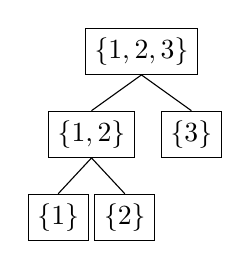
\begin{tikzpicture}[every node/.style={rectangle, draw=black}]
        \Tree [.$\{1,2,3\}$
            [.$\{1,2\}$
                [.$\{1\}$ ]
                [.$\{2\}$ ]
            ]
            [.$\{3\}$ ]
        ]
    \end{tikzpicture}
\end{figure}

Now we have to run the \texttt{FindPairs} (FP) procedure for every inner node. More precisely, we check if the centers $c_l, c_r$ of the bounding boxes of the to child-sets of the inner node are at least $(s+2)\cdot r$ units apart from each other, with $r$ denoting the radius of the bigger enclosing circle of the two bounding boxes. That results in the following list of calls:
\begin{itemize}
    \item FP$(\{1,2\},\{3\}$): $c_1 = (0.5, 0), c_2=p_3, r=0.5$ and $|c_1c_2| \approx 1.118 < 7r = 3.5\:$
    \Lightning
    \begin{itemize}
        \item FP$(\{1\},\{3\})$: $c_1=p_1, c_2=p_3, r=0$ \checkmark
        \item FP$(\{2\},\{3\})$: $c_1=p_2, c_2=p_3, r=0$ \checkmark
    \end{itemize}
    \item FP$(\{1\},\{2\})$: $c_1=p_1, c_2=p_2, r=0$ \checkmark
\end{itemize}
Now we have a WSPD with the following pairs:
\[ \big\{\{1\},\{2\}\big\}, \big\{\{1\},\{3\}\big\}, \big\{\{2\},\{3\}\big\} \]
As every set contains only one point, we can trivially construct the collection of edges $E$:
\[ E = \big\{(1,2),(1,3),(2,3)\} \]
The resulting graph $G=(\{1,2,3\}, E)$ contains a cycle and can therefore be no tree and particularly no MST.
\end{proof}

\section*{Exercise 14}
It suffices to consider the volume of the boxes, because as they are axis-parallel, they can be packed without any gaps. For a box $R$, we get
\[ \text{vol}(R) = \prod_{i=1}^d |b_i - a_i|,\:  \text{ and particularly }\: \text{vol}([0,1]^d) = 1. \]
The number $n$ of boxes fitting in $[0,1]^d$ is therefore given by
\[ n =  \left\lfloor \frac{\text{vol}([0,1]^d)}{\text{vol}(R)} \right\rfloor = \left\lfloor\text{vol}(R)^{-1}\right\rfloor.\]
We know that for every edge $a_ib_i$ we get $l \leq |b_i-a_i| \leq L$ which gives
\[ l^d \leq \text{vol}(R) \leq L^d\]
Thus, a trivial upper bound for $n$ would be
\[ n = \left\lfloor \left(\prod_{i=1}^d |b_i - a_i| \right)^{-1} \right\rfloor \leq \left\lfloor d^{-l} \right\rfloor. \]

\section*{Exercise 15}
Given the following points
\[ p_1=(1,7),\: p_2=(6,5),\: p_3=(3,9),\: p_4=(4,10),\: p_5=(8,3), \]
\[ p_6=(2,8),\: p_7=(5,11),\: p_8=(9,2),\: p_9=(7,2),\: p_10=(12,6) \]
we get the following partial split-trees:
\begin{figure}[h!]
    \centering
    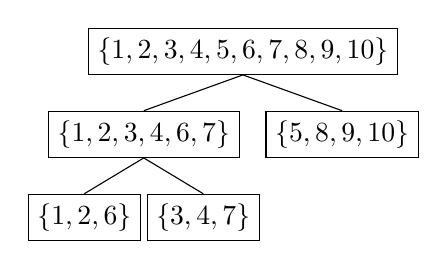
\begin{tikzpicture}[every node/.style={rectangle, draw=black}]
        \Tree [.$\{1,2,3,4,5,6,7,8,9,10\}$
            [.$\{1,2,3,4,6,7\}$
                [.$\{1,2,6\}$ ]
                [.$\{3,4,7\}$ ]
            ]
            [.$\{5,8,9,10\}$ ]
        ]
    \end{tikzpicture}
    
\end{figure}
\begin{figure}[h!]
    \centering
    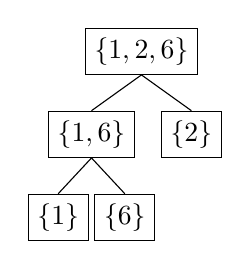
\begin{tikzpicture}[every node/.style={rectangle, draw=black}]
        \Tree [.$\{1,2,6\}$
            [.$\{1,6\}$
                [.$\{1\}$ ]
                [.$\{6\}$ ]
            ]
            [.$\{2\}$ ]
        ]
    \end{tikzpicture}
    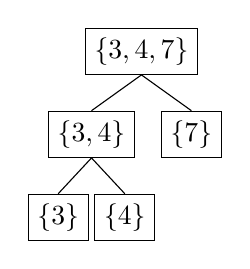
\begin{tikzpicture}[every node/.style={rectangle, draw=black}]
        \Tree [.$\{3,4,7\}$
            [.$\{3,4\}$
                [.$\{3\}$ ]
                [.$\{4\}$ ]
            ]
            [.$\{7\}$ ]
        ]
    \end{tikzpicture}
    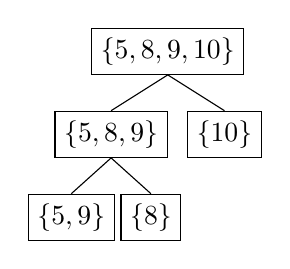
\begin{tikzpicture}[every node/.style={rectangle, draw=black}]
        \Tree [.$\{5,8,9,10\}$
            [.$\{5,8,9\}$
                [.$\{5,9\}$ ]
                [.$\{8\}$ ]
            ]
            [.$\{10\}$ ]
        ]
    \end{tikzpicture}
    
\end{figure}

\begin{figure}[h!]
    \centering
    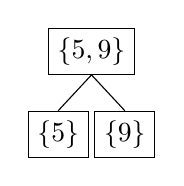
\begin{tikzpicture}[every node/.style={rectangle, draw=black}]
        \Tree [.$\{5,9\}$
            [.$\{5\}$ ]
            [.$\{9\}$ ]
        ]
    \end{tikzpicture}
    
\end{figure}

In this example with $n=10$, we used 5 recursion steps, which is approximately $1.5\cdot \log_2(n)$. Moreover, we get the following number of steps (walking from both sides of the sorted list) for each partial split-tree $T(S')$, where $S'$ denotes the root of the tree:
\begin{itemize}
    \item $T(\{1,2,3,4,5,7,8,9,10\}) = 4 + 3 = 7$
    \item $T(\{1,2,6\}) = 1 + 1$
    \item $T(\{3,4,7\}) = 1 + 1$
    \item $T(\{5,8,9,10\}) = 1 + 1$
    \item $T(\{5,9\}) = 1$.
\end{itemize}
Observe that we require less than $n$ steps for finding the split in each direction and only need $2\cdot n$ steps ($d=2$) to reconstruct the sorted list along all dimensions in each recursion step.

\end{document}